\subsection{Eerste- en tweedegraadsfuncties}
\label{sec:eerste_tweede}

\subsubsection{Constante functies}

\begin{definitie}
	Functievoorschrift: $f(x)=a$ met $a\in\mathbb{R}$
\end{definitie}

%\uline{Voorbeeld}: $f(x)=2$

\textbf{Grafische voorstelling van de constante functie}
met vergelijking $f(x)=a$ is een horizontale rechte, waarbij de $y$-as
wordt gesneden in het punt $(0,a)$.

%Alle afgeleiden zijn overal nul, er zijn geen extrema, geen
%buigpunten...

Tekenverloop: 

\begin{tabel}{Tekenverloop van een constante functie}
	\begin{tabular}{c||c}
		$x$ & \\
		\hline 
		$f(x)$ & teken van $a$\\
	\end{tabular}
	\label{tab:ct}
\end{tabel}


\begin{voorbeeld}
	Gegeven de functie: $f(x)=\frac{1}{2}$. 
%TODO figuur

\begin{figure}[h]
	\centering          
	\tikzsetfigurename{Fig_module_2_1_4_constante_functie}
\begin{tikzpicture}

% Styles
\tikzstyle{axes}=[]
\tikzstyle help lines=[color=blue!50,very thin,dotted]


%%%%%%%%%%%%%%%%%%%%%%%%%%%%%%%%
%		GRID
%%%%%%%%%%%%%%%%%%%%%%%%%%%%%%%%

\draw[style=help lines,step=1cm] (-3.9,-2.9) grid (3.9,2.9);



%%%%%%%%%%%%%%%%%%%%%%%%%%%%%%%%
%		ASSENSTELSEL
%%%%%%%%%%%%%%%%%%%%%%%%%%%%%%%%

\draw[->] (-5,0) -- (5,0) node[right] {$x$};
\draw[->] (0,-3) -- (0,3) node[left]{$y$};

%\draw[fill,cyan](1,1)circle [radius=0.025];

%\draw[red,cap=rect, loosely dashed, ultra thick, domain=-2:2] plot (\x, {(\x*\x-1)+0.05}) node[above,yshift=-.7cm, right]{};

%%%%%%%%%%%%%%%%%%%%%%%%%%%%%%%%
%legende
%%%%%%%%%%%%%%%%%%%%%%%%%%%%%%%%
%\tkzDefPoint(0.5,3.5){A}
%\tkzDefPoint(1,3.5){B}
%\tkzLabelPoint[right,xshift=+0.1cm](B){${\color{cyan}f(x)=|x^2-1|}$}
%\tkzDrawSegment[cyan,ultra thick](A,B)

%\tkzDefPoint(0.5,3.2){C}
%\tkzDefPoint(1,3.2){D}
%\tkzLabelPoint[right,xshift=+0.1cm](D){${\color{red}e(x)=x^2-1}$}
%\tkzDrawSegment[red,cap=rect, loosely dashed, ultra thick](C,D)


%%%%%%%%%%%%%%%%%%%%%%%%%%%%%%%%
%getallen op de x-as en lijntjes
%%%%%%%%%%%%%%%%%%%%%%%%%%%%%%%%   
\foreach \x/\xtext in {-4,-3,-2,-1,0,1,2,3,4}
	\draw[xshift=\x cm] (0pt,1pt) -- (0pt,0pt) node[below,fill=white]
	{$\xtext$};,3
	
%getallen op de y-as en lijntjes  
%BEGIN LUS
\foreach \y/\ytext in {-2,-1,1,2}
	\draw[yshift=\y cm] (1pt,0pt) -- (0pt,0pt) node[left,fill=white]
	{$\ytext$}; %EINDE LUS



%%%%%%%%%%%%%%%%%%%%%%%%%%%%%%%%
%		GRAFIEKEN
%%%%%%%%%%%%%%%%%%%%%%%%%%%%%%%%
%\draw[cyan,cap=rect,thick, domain=-6:6] plot (\x, \x) node[above, right]{${\color{cyan}y=x}$};


\draw[teal,cap=rect,line width=4, opacity=.5, domain=-5:5] plot (\x, {
	0.5		% <- plaats het functievoorschrift hier
}) node[opacity=1,above]{};


 
%node[blue]{stijgen} 
%\draw[cyan,cap=rect,ultra thick, domain=2.25:6] plot (\x, {(\x-2)^(-1)}) node[above,yshift=+0.5cm,left]{$\color{cyan} y=\frac{1}{x-2}$};


%\draw[cyan,cap=rect,ultra thick, domain=-7:1.9] plot (\x, {exp{\x}}) node[above, right]{${\color{cyan}y=\exp{x}}$};

%%%%%%%%%%%%%%%%%%%%%%%%%%%%%%%%
%		MARKERINGEN
%%%%%%%%%%%%%%%%%%%%%%%%%%%%%%%%
%verticale lijn
%\draw[-o,line width=4,teal, cap=rect,opacity=0.3] (0,-4) -- (0,0.25) node[right] {};
%\draw[line width=4,teal, cap=rect,opacity=0.3] (0,0) -- (0,4.2) node[right] {bld $f$ = $\mathbb{R}_0$};
%horizontale lijn

% \draw[white,fill=blue,opacity=.5] (1,-2) circle [radius=.1]   node[blue, above,xshift=-1.1cm,opacity=1] {buigpunt in $(1,-2)$};


 


\draw[] (0,.5) node[blue,left] {$\frac{1}{2}$};
%\draw[] (1.5,-5) node[blue] {bol of convex};

\end{tikzpicture}
 
	\caption{Voorbeeld constante functie}
	\label{fig:constante_functie}	
\end{figure}
	
 
Grafische voorstelling:
\begin{itemize}
\item het domein van de constante functie is altijd: $\textrm{dom}f=\mathbb{R}$
\item het beeld van deze constante functie is: $\textrm{bld}f=\frac{1}{2}$
\end{itemize}
%\begin{figure}[h]
%\centering{}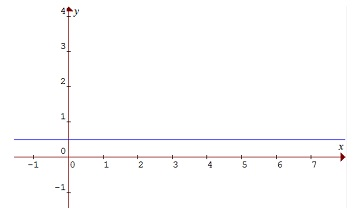
\includegraphics[height=5cm]{2_elem_rekenvaardigheden_B/inputs/constantefuncties.jpg} 
%\caption{Voorbeeld constante functie.}
%\label{fig:ct}
%\end{figure}

Tekenverloop

\begin{center}
\begin{tabular}{c||c}
	$x$ & \\
	\hline 
	$f(x)$ & $+$ \\
\end{tabular}	
\end{center}

\end{voorbeeld}

\subsubsection{Eerstegraadsfuncties of lineaire functies}

\begin{definitie}
	Functievoorschrift: $f(x)=ax+b$ met $a\in\mathbb{R}_{0}$
en $b\in\mathbb{R}$.

\end{definitie}


\begin{voorbeeld}
	 $f(x)=10x+1$ , $f(x)=8-5x$ , $f(x)=3x$
\end{voorbeeld}

Grafische voorstelling van de lineaire functie is een rechte.

%TODO figuur

\begin{figure}[h]
	\centering          
	\begin{tikzpicture}[scale=1,cap=round]

% Styles
\tikzstyle{axes}=[]
\tikzstyle help lines=[color=blue!50,very thin,dotted]


%%%%%%%%%%%%%%%%%%%%%%%%%%%%%%%%
%		GRID
%%%%%%%%%%%%%%%%%%%%%%%%%%%%%%%%

\draw[style=help lines,step=1cm] (-3.9,-2.9) grid (3.9,5.9);



%%%%%%%%%%%%%%%%%%%%%%%%%%%%%%%%
%		ASSENSTELSEL
%%%%%%%%%%%%%%%%%%%%%%%%%%%%%%%%

\draw[->] (-5,0) -- (5,0) node[right] {$x$};
\draw[->] (0,-4) -- (0,7) node[left]{$y$};

%\draw[fill,cyan](1,1)circle [radius=0.025];

%\draw[red,cap=rect, loosely dashed, ultra thick, domain=-2:2] plot (\x, {(\x*\x-1)+0.05}) node[above,yshift=-.7cm, right]{};

%%%%%%%%%%%%%%%%%%%%%%%%%%%%%%%%
%legende
%%%%%%%%%%%%%%%%%%%%%%%%%%%%%%%%
%\tkzDefPoint(0.5,3.5){A}
%\tkzDefPoint(1,3.5){B}
%\tkzLabelPoint[right,xshift=+0.1cm](B){${\color{cyan}f(x)=|x^2-1|}$}
%\tkzDrawSegment[cyan,ultra thick](A,B)

%\tkzDefPoint(0.5,3.2){C}
%\tkzDefPoint(1,3.2){D}
%\tkzLabelPoint[right,xshift=+0.1cm](D){${\color{red}e(x)=x^2-1}$}
%\tkzDrawSegment[red,cap=rect, loosely dashed, ultra thick](C,D)


%%%%%%%%%%%%%%%%%%%%%%%%%%%%%%%%
%getallen op de x-as en lijntjes
%%%%%%%%%%%%%%%%%%%%%%%%%%%%%%%%   
\foreach \x/\xtext in {-4,-3,-2,-1,0,1,2,3,4}
	\draw[xshift=\x cm] (0pt,1pt) -- (0pt,0pt) node[below,fill=white]
	{$\xtext$};,3
	
%getallen op de y-as en lijntjes  
%BEGIN LUS
\foreach \y/\ytext in {-3,-2,-1,1,2,3,4,5,6}
	\draw[yshift=\y cm] (1pt,0pt) -- (0pt,0pt) node[left,fill=white]
	{$\ytext$}; %EINDE LUS



%%%%%%%%%%%%%%%%%%%%%%%%%%%%%%%%
%		GRAFIEKEN
%%%%%%%%%%%%%%%%%%%%%%%%%%%%%%%%
%\draw[cyan,cap=rect,thick, domain=-6:6] plot (\x, \x) node[above, right]{${\color{cyan}y=x}$};


\draw[teal,cap=rect,line width=4, opacity=.5, domain=-3:2] plot (\x, {
	2*\x + 3 		% <- plaats het functievoorschrift hier
}) node[opacity=1,left,pos=1,xshift=-1cm, yshift=+2cm]{$q=3$};
 
%node[blue]{stijgen} 
%\draw[cyan,cap=rect,ultra thick, domain=2.25:6] plot (\x, {(\x-2)^(-1)}) node[above,yshift=+0.5cm,left]{$\color{cyan} y=\frac{1}{x-2}$};


%\draw[cyan,cap=rect,ultra thick, domain=-7:1.9] plot (\x, {exp{\x}}) node[above, right]{${\color{cyan}y=\exp{x}}$};

%%%%%%%%%%%%%%%%%%%%%%%%%%%%%%%%
%		MARKERINGEN
%%%%%%%%%%%%%%%%%%%%%%%%%%%%%%%%
%verticale lijn
%\draw[-o,line width=4,teal, cap=rect,opacity=0.3] (0,-4) -- (0,0.25) node[right] {};
%\draw[line width=4,teal, cap=rect,opacity=0.3] (0,0) -- (0,4.2) node[right] {bld $f$ = $\mathbb{R}_0$};
%horizontale lijn

%horizontale lijn
\draw[->,line width=1,red, cap=rect,opacity=1] (0,3) -- (1,3) node[right] {$1$};
\draw[->,line width=1,red, cap=rect,opacity=1] (1,3) -- (1,5) node[right,pos=0.5] {$m=2$};



% \draw[white,fill=blue,opacity=.5] (1,-2) circle [radius=.1]   node[blue, above,xshift=-1.1cm,opacity=1] {buigpunt in $(1,-2)$};

\draw[] (2,2) node[blue,right] {$y=mx +q$};

\draw[] (2,1) node[blue,right] {$y=2x +3$};

\end{tikzpicture}
 
	\caption{Voorbeeld van een eerstegraadsfunctie}
	\label{fig:eerstegraadsfunctie}	
\end{figure}



%\gewonefiguur{height=5cm}{2_elem_rekenvaardigheden_B/inputs/eerstegraadsfuncties1.jpg}

\begin{itemize}
	\item Het domein van elke lineaire functie is: $\textrm{dom} f = \mathbb{R}$.
	\item Het beeld van deze lineaire functie is: $\textrm{bld} f = \mathbb{R}$.
\end{itemize}

De rechte wordt bepaald door de \textbf{richtingsco\"effici\"ent}
(de \textbf{rico}) \textquoteleft $a$\textquoteright{} en de intercept
\textquoteleft $b$\textquoteright . De rico bepaalt de helling van
de rechte. Als $x$ met 1 eenheid toeneemt, dan neemt $y$ met $a$
eenheden toe. Hoe groter de absolute waarde van de rico $a$, hoe
steiler de rechte.
\begin{itemize}
\item een positieve rico hoort bij een stijgende rechte
\item een negatieve rico hoort bij een dalende rechte
\end{itemize}


%TODO figuur

%M\begin{tabular}{ccc}
	%\hline
%	\begin{tikzpicture}[scale=0.3,cap=round]

% Styles
\tikzstyle{axes}=[]
\tikzstyle help lines=[color=blue!50,very thin,dotted]


%%%%%%%%%%%%%%%%%%%%%%%%%%%%%%%%
%		GRID
%%%%%%%%%%%%%%%%%%%%%%%%%%%%%%%%

\draw[style=help lines,step=1cm] (-3.9,-2.9) grid (3.9,5.9);



%%%%%%%%%%%%%%%%%%%%%%%%%%%%%%%%
%		ASSENSTELSEL
%%%%%%%%%%%%%%%%%%%%%%%%%%%%%%%%

\draw[->] (-5,0) -- (5,0) node[right] {$x$};
\draw[->] (0,-4) -- (0,7) node[left]{$y$};

%\draw[fill,cyan](1,1)circle [radius=0.025];

%\draw[red,cap=rect, loosely dashed, ultra thick, domain=-2:2] plot (\x, {(\x*\x-1)+0.05}) node[above,yshift=-.7cm, right]{};

%%%%%%%%%%%%%%%%%%%%%%%%%%%%%%%%
%legende
%%%%%%%%%%%%%%%%%%%%%%%%%%%%%%%%
%\tkzDefPoint(0.5,3.5){A}
%\tkzDefPoint(1,3.5){B}
%\tkzLabelPoint[right,xshift=+0.1cm](B){${\color{cyan}f(x)=|x^2-1|}$}
%\tkzDrawSegment[cyan,ultra thick](A,B)

%\tkzDefPoint(0.5,3.2){C}
%\tkzDefPoint(1,3.2){D}
%\tkzLabelPoint[right,xshift=+0.1cm](D){${\color{red}e(x)=x^2-1}$}
%\tkzDrawSegment[red,cap=rect, loosely dashed, ultra thick](C,D)


%%%%%%%%%%%%%%%%%%%%%%%%%%%%%%%%
%getallen op de x-as en lijntjes
%%%%%%%%%%%%%%%%%%%%%%%%%%%%%%%%   
\foreach \x/\xtext in {-4,-3,-2,-1,0,1,2,3,4}
	\draw[xshift=\x cm] (0pt,1pt) -- (0pt,0pt) node[below,fill=white]
	{$\xtext$};,3
	
%getallen op de y-as en lijntjes  
%BEGIN LUS
\foreach \y/\ytext in {-3,-2,-1,1,2,3,4,5,6}
	\draw[yshift=\y cm] (1pt,0pt) -- (0pt,0pt) node[left,fill=white]
	{$\ytext$}; %EINDE LUS



%%%%%%%%%%%%%%%%%%%%%%%%%%%%%%%%
%		GRAFIEKEN
%%%%%%%%%%%%%%%%%%%%%%%%%%%%%%%%
%\draw[cyan,cap=rect,thick, domain=-6:6] plot (\x, \x) node[above, right]{${\color{cyan}y=x}$};


\draw[teal,cap=rect,line width=4, opacity=.5, domain=-3:2] plot (\x, {
	2*\x + 3 		% <- plaats het functievoorschrift hier
}) node[opacity=1,left,pos=1,xshift=-1cm, yshift=+2cm]{$q=3$};
 
%node[blue]{stijgen} 
%\draw[cyan,cap=rect,ultra thick, domain=2.25:6] plot (\x, {(\x-2)^(-1)}) node[above,yshift=+0.5cm,left]{$\color{cyan} y=\frac{1}{x-2}$};


%\draw[cyan,cap=rect,ultra thick, domain=-7:1.9] plot (\x, {exp{\x}}) node[above, right]{${\color{cyan}y=\exp{x}}$};

%%%%%%%%%%%%%%%%%%%%%%%%%%%%%%%%
%		MARKERINGEN
%%%%%%%%%%%%%%%%%%%%%%%%%%%%%%%%
%verticale lijn
%\draw[-o,line width=4,teal, cap=rect,opacity=0.3] (0,-4) -- (0,0.25) node[right] {};
%\draw[line width=4,teal, cap=rect,opacity=0.3] (0,0) -- (0,4.2) node[right] {bld $f$ = $\mathbb{R}_0$};
%horizontale lijn

%horizontale lijn



% \draw[white,fill=blue,opacity=.5] (1,-2) circle [radius=.1]   node[blue, above,xshift=-1.1cm,opacity=1] {buigpunt in $(1,-2)$};

\draw[] (2,2) node[blue,right] {$ m > 0 $};



\end{tikzpicture}
 	&\tikzsetfigurename{Fig_module_2_1_4_rico_nul}

\begin{tikzpicture}[scale=0.3,cap=round]

% Styles
\tikzstyle{axes}=[]
\tikzstyle help lines=[color=blue!50,very thin,dotted]


%%%%%%%%%%%%%%%%%%%%%%%%%%%%%%%%
%		GRID
%%%%%%%%%%%%%%%%%%%%%%%%%%%%%%%%

\draw[style=help lines,step=1cm] (-3.9,-2.9) grid (3.9,5.9);



%%%%%%%%%%%%%%%%%%%%%%%%%%%%%%%%
%		ASSENSTELSEL
%%%%%%%%%%%%%%%%%%%%%%%%%%%%%%%%

\draw[->] (-5,0) -- (5,0) node[right] {$x$};
\draw[->] (0,-4) -- (0,7) node[left]{$y$};

%\draw[fill,cyan](1,1)circle [radius=0.025];

%\draw[red,cap=rect, loosely dashed, ultra thick, domain=-2:2] plot (\x, {(\x*\x-1)+0.05}) node[above,yshift=-.7cm, right]{};

%%%%%%%%%%%%%%%%%%%%%%%%%%%%%%%%
%legende
%%%%%%%%%%%%%%%%%%%%%%%%%%%%%%%%
%\tkzDefPoint(0.5,3.5){A}
%\tkzDefPoint(1,3.5){B}
%\tkzLabelPoint[right,xshift=+0.1cm](B){${\color{cyan}f(x)=|x^2-1|}$}
%\tkzDrawSegment[cyan,ultra thick](A,B)

%\tkzDefPoint(0.5,3.2){C}
%\tkzDefPoint(1,3.2){D}
%\tkzLabelPoint[right,xshift=+0.1cm](D){${\color{red}e(x)=x^2-1}$}
%\tkzDrawSegment[red,cap=rect, loosely dashed, ultra thick](C,D)


%%%%%%%%%%%%%%%%%%%%%%%%%%%%%%%%
%getallen op de x-as en lijntjes
%%%%%%%%%%%%%%%%%%%%%%%%%%%%%%%%   
\foreach \x/\xtext in {-4,-3,-2,-1,0,1,2,3,4}
	\draw[xshift=\x cm] (0pt,1pt) -- (0pt,0pt) node[below,fill=white]
	{$\xtext$};,3
	
%getallen op de y-as en lijntjes  
%BEGIN LUS
\foreach \y/\ytext in {-3,-2,-1,1,2,3,4,5,6}
	\draw[yshift=\y cm] (1pt,0pt) -- (0pt,0pt) node[left,fill=white]
	{$\ytext$}; %EINDE LUS



%%%%%%%%%%%%%%%%%%%%%%%%%%%%%%%%
%		GRAFIEKEN
%%%%%%%%%%%%%%%%%%%%%%%%%%%%%%%%
%\draw[cyan,cap=rect,thick, domain=-6:6] plot (\x, \x) node[above, right]{${\color{cyan}y=x}$};


\draw[teal,cap=rect,line width=4, opacity=.5, domain=-5:5] plot (\x, {
	2.3 		% <- plaats het functievoorschrift hier
}) node[opacity=1,left,pos=1,xshift=-1cm, yshift=+2cm]{$q=3$};
 
%node[blue]{stijgen} 
%\draw[cyan,cap=rect,ultra thick, domain=2.25:6] plot (\x, {(\x-2)^(-1)}) node[above,yshift=+0.5cm,left]{$\color{cyan} y=\frac{1}{x-2}$};


%\draw[cyan,cap=rect,ultra thick, domain=-7:1.9] plot (\x, {exp{\x}}) node[above, right]{${\color{cyan}y=\exp{x}}$};

%%%%%%%%%%%%%%%%%%%%%%%%%%%%%%%%
%		MARKERINGEN
%%%%%%%%%%%%%%%%%%%%%%%%%%%%%%%%
%verticale lijn
%\draw[-o,line width=4,teal, cap=rect,opacity=0.3] (0,-4) -- (0,0.25) node[right] {};
%\draw[line width=4,teal, cap=rect,opacity=0.3] (0,0) -- (0,4.2) node[right] {bld $f$ = $\mathbb{R}_0$};
%horizontale lijn

%horizontale lijn





% \draw[white,fill=blue,opacity=.5] (1,-2) circle [radius=.1]   node[blue, above,xshift=-1.1cm,opacity=1] {buigpunt in $(1,-2)$};

\draw[] (2,3) node[blue,right] {$m=0$};



\end{tikzpicture}
  &  \begin{tikzpicture}[scale=0.3,cap=round]

% Styles
\tikzstyle{axes}=[]
\tikzstyle help lines=[color=blue!50,very thin,dotted]


%%%%%%%%%%%%%%%%%%%%%%%%%%%%%%%%
%		GRID
%%%%%%%%%%%%%%%%%%%%%%%%%%%%%%%%

\draw[style=help lines,step=1cm] (-3.9,-2.9) grid (3.9,5.9);



%%%%%%%%%%%%%%%%%%%%%%%%%%%%%%%%
%		ASSENSTELSEL
%%%%%%%%%%%%%%%%%%%%%%%%%%%%%%%%

\draw[->] (-5,0) -- (5,0) node[right] {$x$};
\draw[->] (0,-4) -- (0,7) node[left]{$y$};

%\draw[fill,cyan](1,1)circle [radius=0.025];

%\draw[red,cap=rect, loosely dashed, ultra thick, domain=-2:2] plot (\x, {(\x*\x-1)+0.05}) node[above,yshift=-.7cm, right]{};

%%%%%%%%%%%%%%%%%%%%%%%%%%%%%%%%
%legende
%%%%%%%%%%%%%%%%%%%%%%%%%%%%%%%%
%\tkzDefPoint(0.5,3.5){A}
%\tkzDefPoint(1,3.5){B}
%\tkzLabelPoint[right,xshift=+0.1cm](B){${\color{cyan}f(x)=|x^2-1|}$}
%\tkzDrawSegment[cyan,ultra thick](A,B)

%\tkzDefPoint(0.5,3.2){C}
%\tkzDefPoint(1,3.2){D}
%\tkzLabelPoint[right,xshift=+0.1cm](D){${\color{red}e(x)=x^2-1}$}
%\tkzDrawSegment[red,cap=rect, loosely dashed, ultra thick](C,D)


%%%%%%%%%%%%%%%%%%%%%%%%%%%%%%%%
%getallen op de x-as en lijntjes
%%%%%%%%%%%%%%%%%%%%%%%%%%%%%%%%   
\foreach \x/\xtext in {-4,-3,-2,-1,0,1,2,3,4}
	\draw[xshift=\x cm] (0pt,1pt) -- (0pt,0pt) node[below,fill=white]
	{$\xtext$};,3
	
%getallen op de y-as en lijntjes  
%BEGIN LUS
\foreach \y/\ytext in {-3,-2,-1,1,2,3,4,5,6}
	\draw[yshift=\y cm] (1pt,0pt) -- (0pt,0pt) node[left,fill=white]
	{$\ytext$}; %EINDE LUS



%%%%%%%%%%%%%%%%%%%%%%%%%%%%%%%%
%		GRAFIEKEN
%%%%%%%%%%%%%%%%%%%%%%%%%%%%%%%%
%\draw[cyan,cap=rect,thick, domain=-6:6] plot (\x, \x) node[above, right]{${\color{cyan}y=x}$};


\draw[teal,cap=rect,line width=4, opacity=.5, domain=-1:3] plot (\x, {
	(-2)*\x + 3  		% <- plaats het functievoorschrift hier
}) node[opacity=1,left,pos=1,xshift=-1cm, yshift=+2cm]{$q=3$};
 
%node[blue]{stijgen} 
%\draw[cyan,cap=rect,ultra thick, domain=2.25:6] plot (\x, {(\x-2)^(-1)}) node[above,yshift=+0.5cm,left]{$\color{cyan} y=\frac{1}{x-2}$};


%\draw[cyan,cap=rect,ultra thick, domain=-7:1.9] plot (\x, {exp{\x}}) node[above, right]{${\color{cyan}y=\exp{x}}$};

%%%%%%%%%%%%%%%%%%%%%%%%%%%%%%%%
%		MARKERINGEN
%%%%%%%%%%%%%%%%%%%%%%%%%%%%%%%%
%verticale lijn
%\draw[-o,line width=4,teal, cap=rect,opacity=0.3] (0,-4) -- (0,0.25) node[right] {};
%\draw[line width=4,teal, cap=rect,opacity=0.3] (0,0) -- (0,4.2) node[right] {bld $f$ = $\mathbb{R}_0$};
%horizontale lijn

%horizontale lijn




% \draw[white,fill=blue,opacity=.5] (1,-2) circle [radius=.1]   node[blue, above,xshift=-1.1cm,opacity=1] {buigpunt in $(1,-2)$};

\draw[] (2,2) node[blue,right] {$m<0$};



\end{tikzpicture}
   \\
	%\hline
%\end{tabular}


\begin{figure}[h]
	\centering
	\begin{subfigure}{0.3\textwidth}
	\begin{tikzpicture}[scale=0.3,cap=round]

% Styles
\tikzstyle{axes}=[]
\tikzstyle help lines=[color=blue!50,very thin,dotted]


%%%%%%%%%%%%%%%%%%%%%%%%%%%%%%%%
%		GRID
%%%%%%%%%%%%%%%%%%%%%%%%%%%%%%%%

\draw[style=help lines,step=1cm] (-3.9,-2.9) grid (3.9,5.9);



%%%%%%%%%%%%%%%%%%%%%%%%%%%%%%%%
%		ASSENSTELSEL
%%%%%%%%%%%%%%%%%%%%%%%%%%%%%%%%

\draw[->] (-5,0) -- (5,0) node[right] {$x$};
\draw[->] (0,-4) -- (0,7) node[left]{$y$};

%\draw[fill,cyan](1,1)circle [radius=0.025];

%\draw[red,cap=rect, loosely dashed, ultra thick, domain=-2:2] plot (\x, {(\x*\x-1)+0.05}) node[above,yshift=-.7cm, right]{};

%%%%%%%%%%%%%%%%%%%%%%%%%%%%%%%%
%legende
%%%%%%%%%%%%%%%%%%%%%%%%%%%%%%%%
%\tkzDefPoint(0.5,3.5){A}
%\tkzDefPoint(1,3.5){B}
%\tkzLabelPoint[right,xshift=+0.1cm](B){${\color{cyan}f(x)=|x^2-1|}$}
%\tkzDrawSegment[cyan,ultra thick](A,B)

%\tkzDefPoint(0.5,3.2){C}
%\tkzDefPoint(1,3.2){D}
%\tkzLabelPoint[right,xshift=+0.1cm](D){${\color{red}e(x)=x^2-1}$}
%\tkzDrawSegment[red,cap=rect, loosely dashed, ultra thick](C,D)


%%%%%%%%%%%%%%%%%%%%%%%%%%%%%%%%
%getallen op de x-as en lijntjes
%%%%%%%%%%%%%%%%%%%%%%%%%%%%%%%%   
\foreach \x/\xtext in {-4,-3,-2,-1,0,1,2,3,4}
	\draw[xshift=\x cm] (0pt,1pt) -- (0pt,0pt) node[below,fill=white]
	{$\xtext$};,3
	
%getallen op de y-as en lijntjes  
%BEGIN LUS
\foreach \y/\ytext in {-3,-2,-1,1,2,3,4,5,6}
	\draw[yshift=\y cm] (1pt,0pt) -- (0pt,0pt) node[left,fill=white]
	{$\ytext$}; %EINDE LUS



%%%%%%%%%%%%%%%%%%%%%%%%%%%%%%%%
%		GRAFIEKEN
%%%%%%%%%%%%%%%%%%%%%%%%%%%%%%%%
%\draw[cyan,cap=rect,thick, domain=-6:6] plot (\x, \x) node[above, right]{${\color{cyan}y=x}$};


\draw[teal,cap=rect,line width=4, opacity=.5, domain=-3:2] plot (\x, {
	2*\x + 3 		% <- plaats het functievoorschrift hier
}) node[opacity=1,left,pos=1,xshift=-1cm, yshift=+2cm]{$q=3$};
 
%node[blue]{stijgen} 
%\draw[cyan,cap=rect,ultra thick, domain=2.25:6] plot (\x, {(\x-2)^(-1)}) node[above,yshift=+0.5cm,left]{$\color{cyan} y=\frac{1}{x-2}$};


%\draw[cyan,cap=rect,ultra thick, domain=-7:1.9] plot (\x, {exp{\x}}) node[above, right]{${\color{cyan}y=\exp{x}}$};

%%%%%%%%%%%%%%%%%%%%%%%%%%%%%%%%
%		MARKERINGEN
%%%%%%%%%%%%%%%%%%%%%%%%%%%%%%%%
%verticale lijn
%\draw[-o,line width=4,teal, cap=rect,opacity=0.3] (0,-4) -- (0,0.25) node[right] {};
%\draw[line width=4,teal, cap=rect,opacity=0.3] (0,0) -- (0,4.2) node[right] {bld $f$ = $\mathbb{R}_0$};
%horizontale lijn

%horizontale lijn



% \draw[white,fill=blue,opacity=.5] (1,-2) circle [radius=.1]   node[blue, above,xshift=-1.1cm,opacity=1] {buigpunt in $(1,-2)$};

\draw[] (2,2) node[blue,right] {$ m > 0 $};



\end{tikzpicture}
 
	\caption{}
	\label{fig:rico_pos}	
	\end{subfigure}
	\begin{subfigure}{0.3\textwidth}
	\tikzsetfigurename{Fig_module_2_1_4_rico_nul}

\begin{tikzpicture}[scale=0.3,cap=round]

% Styles
\tikzstyle{axes}=[]
\tikzstyle help lines=[color=blue!50,very thin,dotted]


%%%%%%%%%%%%%%%%%%%%%%%%%%%%%%%%
%		GRID
%%%%%%%%%%%%%%%%%%%%%%%%%%%%%%%%

\draw[style=help lines,step=1cm] (-3.9,-2.9) grid (3.9,5.9);



%%%%%%%%%%%%%%%%%%%%%%%%%%%%%%%%
%		ASSENSTELSEL
%%%%%%%%%%%%%%%%%%%%%%%%%%%%%%%%

\draw[->] (-5,0) -- (5,0) node[right] {$x$};
\draw[->] (0,-4) -- (0,7) node[left]{$y$};

%\draw[fill,cyan](1,1)circle [radius=0.025];

%\draw[red,cap=rect, loosely dashed, ultra thick, domain=-2:2] plot (\x, {(\x*\x-1)+0.05}) node[above,yshift=-.7cm, right]{};

%%%%%%%%%%%%%%%%%%%%%%%%%%%%%%%%
%legende
%%%%%%%%%%%%%%%%%%%%%%%%%%%%%%%%
%\tkzDefPoint(0.5,3.5){A}
%\tkzDefPoint(1,3.5){B}
%\tkzLabelPoint[right,xshift=+0.1cm](B){${\color{cyan}f(x)=|x^2-1|}$}
%\tkzDrawSegment[cyan,ultra thick](A,B)

%\tkzDefPoint(0.5,3.2){C}
%\tkzDefPoint(1,3.2){D}
%\tkzLabelPoint[right,xshift=+0.1cm](D){${\color{red}e(x)=x^2-1}$}
%\tkzDrawSegment[red,cap=rect, loosely dashed, ultra thick](C,D)


%%%%%%%%%%%%%%%%%%%%%%%%%%%%%%%%
%getallen op de x-as en lijntjes
%%%%%%%%%%%%%%%%%%%%%%%%%%%%%%%%   
\foreach \x/\xtext in {-4,-3,-2,-1,0,1,2,3,4}
	\draw[xshift=\x cm] (0pt,1pt) -- (0pt,0pt) node[below,fill=white]
	{$\xtext$};,3
	
%getallen op de y-as en lijntjes  
%BEGIN LUS
\foreach \y/\ytext in {-3,-2,-1,1,2,3,4,5,6}
	\draw[yshift=\y cm] (1pt,0pt) -- (0pt,0pt) node[left,fill=white]
	{$\ytext$}; %EINDE LUS



%%%%%%%%%%%%%%%%%%%%%%%%%%%%%%%%
%		GRAFIEKEN
%%%%%%%%%%%%%%%%%%%%%%%%%%%%%%%%
%\draw[cyan,cap=rect,thick, domain=-6:6] plot (\x, \x) node[above, right]{${\color{cyan}y=x}$};


\draw[teal,cap=rect,line width=4, opacity=.5, domain=-5:5] plot (\x, {
	2.3 		% <- plaats het functievoorschrift hier
}) node[opacity=1,left,pos=1,xshift=-1cm, yshift=+2cm]{$q=3$};
 
%node[blue]{stijgen} 
%\draw[cyan,cap=rect,ultra thick, domain=2.25:6] plot (\x, {(\x-2)^(-1)}) node[above,yshift=+0.5cm,left]{$\color{cyan} y=\frac{1}{x-2}$};


%\draw[cyan,cap=rect,ultra thick, domain=-7:1.9] plot (\x, {exp{\x}}) node[above, right]{${\color{cyan}y=\exp{x}}$};

%%%%%%%%%%%%%%%%%%%%%%%%%%%%%%%%
%		MARKERINGEN
%%%%%%%%%%%%%%%%%%%%%%%%%%%%%%%%
%verticale lijn
%\draw[-o,line width=4,teal, cap=rect,opacity=0.3] (0,-4) -- (0,0.25) node[right] {};
%\draw[line width=4,teal, cap=rect,opacity=0.3] (0,0) -- (0,4.2) node[right] {bld $f$ = $\mathbb{R}_0$};
%horizontale lijn

%horizontale lijn





% \draw[white,fill=blue,opacity=.5] (1,-2) circle [radius=.1]   node[blue, above,xshift=-1.1cm,opacity=1] {buigpunt in $(1,-2)$};

\draw[] (2,3) node[blue,right] {$m=0$};



\end{tikzpicture}
 
	\caption{}
	\label{fig:rico_nul}	
	\end{subfigure}
	\begin{subfigure}{0.3\textwidth}
	\begin{tikzpicture}[scale=0.3,cap=round]

% Styles
\tikzstyle{axes}=[]
\tikzstyle help lines=[color=blue!50,very thin,dotted]


%%%%%%%%%%%%%%%%%%%%%%%%%%%%%%%%
%		GRID
%%%%%%%%%%%%%%%%%%%%%%%%%%%%%%%%

\draw[style=help lines,step=1cm] (-3.9,-2.9) grid (3.9,5.9);



%%%%%%%%%%%%%%%%%%%%%%%%%%%%%%%%
%		ASSENSTELSEL
%%%%%%%%%%%%%%%%%%%%%%%%%%%%%%%%

\draw[->] (-5,0) -- (5,0) node[right] {$x$};
\draw[->] (0,-4) -- (0,7) node[left]{$y$};

%\draw[fill,cyan](1,1)circle [radius=0.025];

%\draw[red,cap=rect, loosely dashed, ultra thick, domain=-2:2] plot (\x, {(\x*\x-1)+0.05}) node[above,yshift=-.7cm, right]{};

%%%%%%%%%%%%%%%%%%%%%%%%%%%%%%%%
%legende
%%%%%%%%%%%%%%%%%%%%%%%%%%%%%%%%
%\tkzDefPoint(0.5,3.5){A}
%\tkzDefPoint(1,3.5){B}
%\tkzLabelPoint[right,xshift=+0.1cm](B){${\color{cyan}f(x)=|x^2-1|}$}
%\tkzDrawSegment[cyan,ultra thick](A,B)

%\tkzDefPoint(0.5,3.2){C}
%\tkzDefPoint(1,3.2){D}
%\tkzLabelPoint[right,xshift=+0.1cm](D){${\color{red}e(x)=x^2-1}$}
%\tkzDrawSegment[red,cap=rect, loosely dashed, ultra thick](C,D)


%%%%%%%%%%%%%%%%%%%%%%%%%%%%%%%%
%getallen op de x-as en lijntjes
%%%%%%%%%%%%%%%%%%%%%%%%%%%%%%%%   
\foreach \x/\xtext in {-4,-3,-2,-1,0,1,2,3,4}
	\draw[xshift=\x cm] (0pt,1pt) -- (0pt,0pt) node[below,fill=white]
	{$\xtext$};,3
	
%getallen op de y-as en lijntjes  
%BEGIN LUS
\foreach \y/\ytext in {-3,-2,-1,1,2,3,4,5,6}
	\draw[yshift=\y cm] (1pt,0pt) -- (0pt,0pt) node[left,fill=white]
	{$\ytext$}; %EINDE LUS



%%%%%%%%%%%%%%%%%%%%%%%%%%%%%%%%
%		GRAFIEKEN
%%%%%%%%%%%%%%%%%%%%%%%%%%%%%%%%
%\draw[cyan,cap=rect,thick, domain=-6:6] plot (\x, \x) node[above, right]{${\color{cyan}y=x}$};


\draw[teal,cap=rect,line width=4, opacity=.5, domain=-1:3] plot (\x, {
	(-2)*\x + 3  		% <- plaats het functievoorschrift hier
}) node[opacity=1,left,pos=1,xshift=-1cm, yshift=+2cm]{$q=3$};
 
%node[blue]{stijgen} 
%\draw[cyan,cap=rect,ultra thick, domain=2.25:6] plot (\x, {(\x-2)^(-1)}) node[above,yshift=+0.5cm,left]{$\color{cyan} y=\frac{1}{x-2}$};


%\draw[cyan,cap=rect,ultra thick, domain=-7:1.9] plot (\x, {exp{\x}}) node[above, right]{${\color{cyan}y=\exp{x}}$};

%%%%%%%%%%%%%%%%%%%%%%%%%%%%%%%%
%		MARKERINGEN
%%%%%%%%%%%%%%%%%%%%%%%%%%%%%%%%
%verticale lijn
%\draw[-o,line width=4,teal, cap=rect,opacity=0.3] (0,-4) -- (0,0.25) node[right] {};
%\draw[line width=4,teal, cap=rect,opacity=0.3] (0,0) -- (0,4.2) node[right] {bld $f$ = $\mathbb{R}_0$};
%horizontale lijn

%horizontale lijn




% \draw[white,fill=blue,opacity=.5] (1,-2) circle [radius=.1]   node[blue, above,xshift=-1.1cm,opacity=1] {buigpunt in $(1,-2)$};

\draw[] (2,2) node[blue,right] {$m<0$};



\end{tikzpicture}
 
	\caption{}
	\label{fig:rico_neg}	
\end{subfigure}
\caption{Het teken van de richtingscoëfficiënt bepaalt of de rechte stijgt, constant is of daalt.}
\label{fig:rico}

\end{figure}
  


%\gewonefiguur{width=\linewidth}{2_elem_rekenvaardigheden_B/inputs/eerstegraadsfuncties2.jpg}

Een rechte evenwijdig met de $x$-as heeft een rico gelijk
aan 0. Dit is in feite de constante functie $f(x)=b$.

Een rechte evenwijdig met de $y$-as heeft geen rico (in
dit geval zou $m=\infty$ moeten zijn). 

Nulpunten: het snijpunt met de $x$-as is het
punt $(-\frac{b}{a},0)$.

%\uline{De eerste afgeleide} van $f(x)$ is $f^{'}(x)=(mx+b)^{'}=m$.
%Dit betekent dat de eerste afgeleide ons meteen vertelt of het om
%een stijgende of een dalende rechte gaat.
%
%Er zijn geen extrema, geen buigpunten...

Tekenverloop: 
\begin{tabel}{Tekenverloop voor $a>0$}
	\centering\begin{tabular}{c||c|c|c}
		$x$ &  & $-\frac{b}{a}$ & \\
		\hline 
		$f(x)$ & - & 0 & +\\
	\end{tabular}
\end{tabel}

\begin{tabel}{Tekenverloop voor $a<0$.}
	\centering\begin{tabular}{c||c|c|c}
		$x$ &  & $-\frac{b}{a}$ & \\
		\hline 
		$f(x)$ & + & 0 & -\\
	\end{tabular}
	\label{tab:eerst_akl0}
\end{tabel}

\begin{voorbeeld}
	Gegeven de functie: $f(x)=-2x+3$.
	

Grafische voorstelling:
\begin{itemize}
\item het domein van elke lineaire functie is: $\textrm{dom}f=\mathbb{R}$
\item het beeld van deze lineaire functie is: $\textrm{bld}f=\mathbb{R}$
\end{itemize}
%TODO figuur vervangen 


\begin{figure}[h]
	\centering          
	
		\tikzsetfigurename{Fig_module_2_1_4_eerstegraadsfunctie_3}

\begin{tikzpicture}[scale=.5,cap=round]

% Styles
\tikzstyle{axes}=[]
\tikzstyle help lines=[color=blue!50,very thin,dotted]


%%%%%%%%%%%%%%%%%%%%%%%%%%%%%%%%
%		GRID
%%%%%%%%%%%%%%%%%%%%%%%%%%%%%%%%

\draw[style=help lines,step=1cm] (-3.9,-2.9) grid (3.9,5.9);



%%%%%%%%%%%%%%%%%%%%%%%%%%%%%%%%
%		ASSENSTELSEL
%%%%%%%%%%%%%%%%%%%%%%%%%%%%%%%%

\draw[->] (-5,0) -- (5,0) node[right] {$x$};
\draw[->] (0,-4) -- (0,7) node[left]{$y$};

%\draw[fill,cyan](1,1)circle [radius=0.025];

%\draw[red,cap=rect, loosely dashed, ultra thick, domain=-2:2] plot (\x, {(\x*\x-1)+0.05}) node[above,yshift=-.7cm, right]{};

%%%%%%%%%%%%%%%%%%%%%%%%%%%%%%%%
%legende
%%%%%%%%%%%%%%%%%%%%%%%%%%%%%%%%
%\tkzDefPoint(0.5,3.5){A}
%\tkzDefPoint(1,3.5){B}
%\tkzLabelPoint[right,xshift=+0.1cm](B){${\color{cyan}f(x)=|x^2-1|}$}
%\tkzDrawSegment[cyan,ultra thick](A,B)

%\tkzDefPoint(0.5,3.2){C}
%\tkzDefPoint(1,3.2){D}
%\tkzLabelPoint[right,xshift=+0.1cm](D){${\color{red}e(x)=x^2-1}$}
%\tkzDrawSegment[red,cap=rect, loosely dashed, ultra thick](C,D)


%%%%%%%%%%%%%%%%%%%%%%%%%%%%%%%%
%getallen op de x-as en lijntjes
%%%%%%%%%%%%%%%%%%%%%%%%%%%%%%%%   
\foreach \x/\xtext in {-4,-3,-2,-1,0,1,2,3,4}
	\draw[xshift=\x cm] (0pt,1pt) -- (0pt,0pt) node[below,fill=white]
	{$\xtext$};,3
	
%getallen op de y-as en lijntjes  
%BEGIN LUS
\foreach \y/\ytext in {-3,-2,-1,1,2,3,4,5,6}
	\draw[yshift=\y cm] (1pt,0pt) -- (0pt,0pt) node[left,fill=white]
	{$\ytext$}; %EINDE LUS



%%%%%%%%%%%%%%%%%%%%%%%%%%%%%%%%
%		GRAFIEKEN
%%%%%%%%%%%%%%%%%%%%%%%%%%%%%%%%
%\draw[cyan,cap=rect,thick, domain=-6:6] plot (\x, \x) node[above, right]{${\color{cyan}y=x}$};


\draw[teal,cap=rect,line width=4, opacity=.5, domain=-2:3] plot (\x, {
	(-2)*\x + 3  		% <- plaats het functievoorschrift hier
}) node[opacity=1,left,pos=1,xshift=-1cm, yshift=+2cm]{};
 
%node[blue]{stijgen} 
%\draw[cyan,cap=rect,ultra thick, domain=2.25:6] plot (\x, {(\x-2)^(-1)}) node[above,yshift=+0.5cm,left]{$\color{cyan} y=\frac{1}{x-2}$};


%\draw[cyan,cap=rect,ultra thick, domain=-7:1.9] plot (\x, {exp{\x}}) node[above, right]{${\color{cyan}y=\exp{x}}$};

%%%%%%%%%%%%%%%%%%%%%%%%%%%%%%%%
%		MARKERINGEN
%%%%%%%%%%%%%%%%%%%%%%%%%%%%%%%%
%verticale lijn
%\draw[-o,line width=4,teal, cap=rect,opacity=0.3] (0,-4) -- (0,0.25) node[right] {};
%\draw[line width=4,teal, cap=rect,opacity=0.3] (0,0) -- (0,4.2) node[right] {bld $f$ = $\mathbb{R}_0$};
%horizontale lijn

%horizontale lijn
%\draw[->,line width=1,red, cap=rect,opacity=1] (0,3) -- (1,3) node[right] {$1$};
%\draw[->,line width=1,red, cap=rect,opacity=1] (1,3) -- (1,5) node[right,pos=0.5] {$m=2$};



% \draw[white,fill=blue,opacity=.5] (1,-2) circle [radius=.1]   node[blue, above,xshift=-1.1cm,opacity=1] {buigpunt in $(1,-2)$};

\draw[] (0.5,3) node[blue,right] {$b$};

\draw[fill,cyan](1.5,0)circle [radius=0.025];
\draw[] (1,-2) node[blue,right] {$-\frac{a}{b}$};

\end{tikzpicture}
 
	\caption{Voorbeeld van de grafische voorstelling van een eerstegraadsfunctie}
	\label{fig:eerstegraadsfunctie_3}	
\end{figure}

%\gewonefiguur{height=5cm}{2_elem_rekenvaardigheden_B/inputs/eerstegraadsfuncties3.jpg}

%\begin{figure}[h]
%\centering{}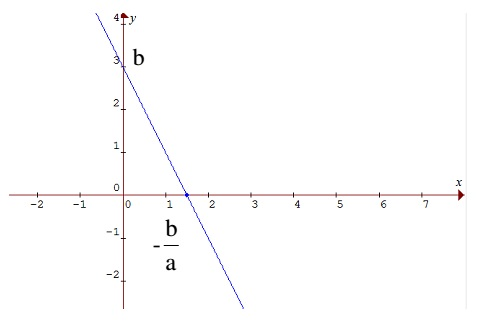
\includegraphics[height=5cm]{2_elem_rekenvaardigheden_B/inputs/eerstegraadsfuncties3.jpg}
%\caption{Voorbeeld grafische voorstelling van de eerstegraadfunctie.}
%\label{fig:eerste_vb_graf} 
%\end{figure}

Nulpunten:

We lossen de vergelijking $y=f(x)=-2x+3=0$ op en vinden:
$x=\frac{3}{2}$. Het snijpunt met de $x$-as is het punt $(\frac{3}{2},0)$.

Tekenverloop: zie Tabel \ref{tab:eerste_vb}.

\begin{tabel}{Voorbeeld eerstegraadsfunctie: tekenverloop}
\begin{tabular}{c||c|c|c}
	$x$ &  & $\frac{3}{2}$ & \\
	\hline 
	$f(x)$ & $+$ & 0 & $-$\\
\end{tabular}
\label{tab:eerste_vb}	
\end{tabel}

\end{voorbeeld}

\subsubsection{Tweedegraadsfuncties of kwadratische functies}



\begin{definitie}
	Functievoorschrift: $f(x)=ax^{2}+bx+c$ met $a\in\mathbb{R}_{0}$
en $b,c\in\mathbb{R}$ 

\end{definitie}

\begin{voorbeeld}
	$f(x)=3x^{2}+10x+1$ , $f(x)=-2x^{2}+5$
, $f(x)=x^{2}$
\end{voorbeeld}

Grafische voorstelling van de kwadratische functie
is een parabool.
%TODO figuur  vervangen 
\gewonefiguur{width=.7\linewidth}{2_elem_rekenvaardigheden_B/inputs/tweedegraadsfuncties1.jpg}

%\begin{figure}[h]
%\centering{}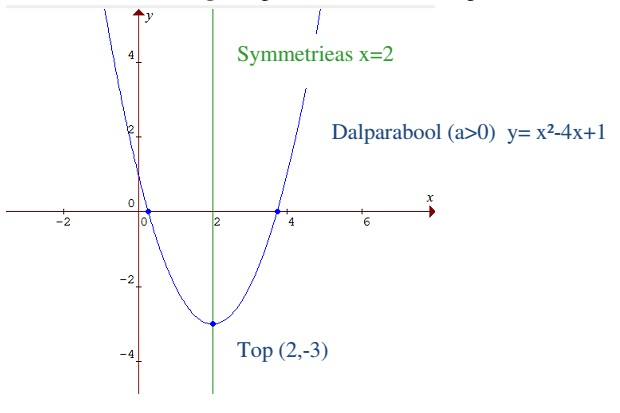
\includegraphics[width=.7\linewidth]{2_elem_rekenvaardigheden_B/inputs/tweedegraadsfuncties1.jpg}
%\caption{Grafische voorstelling van een tweedegraadsfunctie.}
%\label{fig:tweede} 
%\end{figure}

\begin{itemize}
\item als $a>0$ is de top van de \textbf{dalparabool} het minimum
\item als $a<0$ is de top van de \textbf{bergparabool} het maximum
\end{itemize}
Hoe groter de absolute waarde van $a$, hoe smaller de opening
van de parabool is.

De verticale lijn door de top is de \textbf{symmetrieas}.
De vergelijking van de symmetrieas is: $x=-\frac{b}{2a}$ 

Het laagste punt van een dalparabool of het hoogste punt
van een bergparabool heet de \textbf{top} van de parabool. De top
is het snijpunt van de parabool met de verticale symmetrieas. De co\"ordinaten
van de top zijn dus $(-\frac{b}{2a},y)$. De $y$-waarde vinden we
door de gevonden $x$-waarde in het functievoorschrift $f(x)$ in
te vullen, dus $y=f(-\frac{b}{2a})$ .

Nulpunten: stellen we $y=f(x)=ax^{2}+bx+c=0$
(in dat geval spreken we van de \textbf{vierkantsvergelijking}), dan
vinden we de snijpunten met de $x$-as. Hiervoor moeten we dus de
(vierkants)vergelijking $ax^{2}+bx+c=0$ oplossen. Daarvoor bepaal
je best eerst de \textbf{discriminant} $D=b^{2}-4ac$ (van de abc
formule). Met de discriminant bepaal je het aantal snijpunten van
de kwadratische functie met de $x$-as.
\begin{itemize}
\item als $D>0$ , dan heeft de vergelijking twee oplossing: $x_{1}=\frac{-b+\sqrt{D}}{2a}$
en $x_{2}=\frac{-b-\sqrt{D}}{2a}$. De parabool snijdt de $x$-as
op twee plaatsen.
\item als $D=0$ , dan heeft de vergelijking \'e\'en oplossing: $x_{1}=x_{2}=-\frac{b}{2a}$.
De parabool raakt met zijn top de $x$-as in \'e\'en punt.
\item als $D<0$ , dan heeft de vergelijking geen re\"ele oplossingen. De
parabool ligt ofwel boven ofwel onder de $x$-as.
\end{itemize}

%TODO figuur vervangen 
\gewonefiguur{scale=0.8}{2_elem_rekenvaardigheden_B/inputs/tweedegraadsfuncties2.jpg}

%\begin{figure}[h]
%\centering{}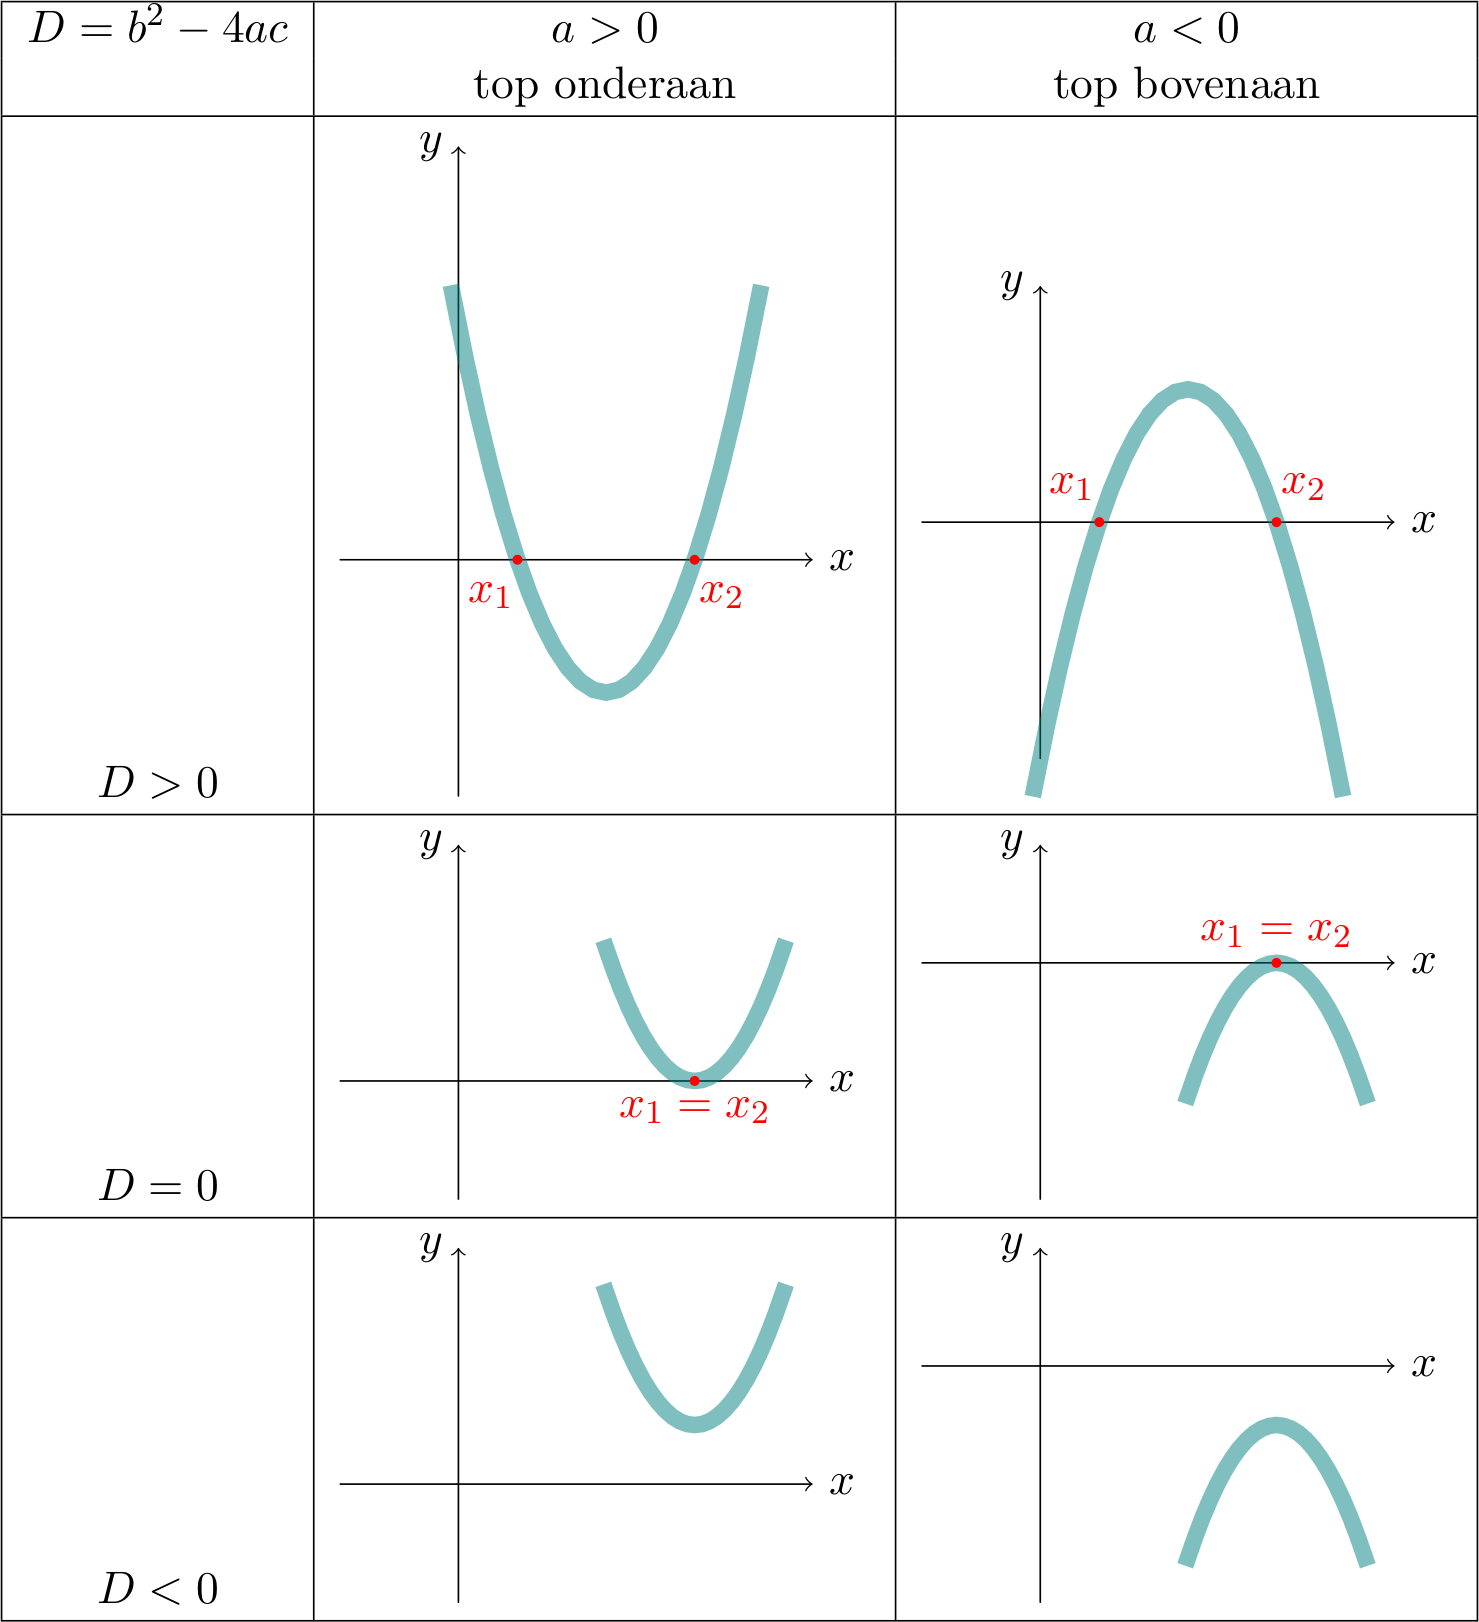
\includegraphics[scale=0.8]{2_elem_rekenvaardigheden_B/inputs/tweedegraadsfuncties2.jpg} 
%\caption{Grafische voorstelling van tweedegraadsfuncties voor verschillende waarden van $a$ en $D$.}
%\label{fig:tweede:gevallen}
%\end{figure}


%\uline{Opmerking}: stellen we de eerste afgeleide gelijk
%aan nul, dan vinden we de $x$-co\"ordinaat van de top: $f^{'}(x)=(ax^{2}+bx+c)^{'}=2ax+b=0$
%of $x=-\frac{b}{2a}$ . Het teken van de eerste afgeleide zegt ons
%of de functie (links en rechts van de top) stijgt of daalt. Tenslotte,
%het teken van de tweede afgeleide $f^{''}(x)=(2ax+b)^{'}=2a$, m.a.w.
%het teken van $a$ , zegt ons of het om een dal- of bergparabool gaat.

Tekenverloop:

\begin{itemize}
\item Als $D>0$ \\
\begin{center}
	\begin{tabular}{c||c|c|c|c|c}
$x$ &  & $x_{1}$ &  & $x_{2}$ & \\
\hline 
$f(x)$ & teken van $a$ & 0 & tegengesteld teken van $a$ & 0 & teken van $a$\\
\end{tabular}
\end{center}
\item Als $D=0$ \\
\begin{center}
	\begin{tabular}{c||c|c|c}
	$x$ &  & $x_{1}=x_{2}$ & \\
	\hline 
	$f(x)$ & teken van $a$ & 0 & teken van $a$\\
\end{tabular}
\end{center}
\item Als $D<0$ \\
\begin{center}
	\begin{tabular}{c||c}
$x$ & \\
\hline 
$f(x)$ & teken van $a$\\
\end{tabular}
\end{center}
\end{itemize}
%\begin{table}[h]
%\centering
%\caption{Algemeen tekenverloop van een tweedegraadsfunctie voor $D>0$}
%\end{table}
%\begin{tabular}{c|c}
%$D=0$ & %
%\begin{tabular}{c||c|c|c}
%$x$ &  & $x_{1}=x_{2}$ & \\
%\hline 
%\hline 
%$f(x)$ & teken van $a$ & 0 & teken van $a$\\
%\end{tabular}\\
% & \\
%\hline 
% & \\
%$D>0$ & %
%\begin{tabular}{c||c|c|c|c|c}
%$x$ &  & $x_{1}$ &  & $x_{2}$ & \\
%\hline 
%\hline 
%$f(x)$ & teken van $a$ & 0 & tegengesteld teken van $a$ & 0 & teken van $a$\\
%\end{tabular}\\
% & \\
%\hline 
% & \\
%$D<0$ & %
%\begin{tabular}{c||c}
%$x$ & \\
%\hline 
%\hline 
%$f(x)$ & teken van $a$\\
%\end{tabular}\\
%\end{tabular}


\begin{voorbeeld}
	Gegeven de functie $f$ met voorschrift: $f(x)=-x^{2}-5x+6$ 

Grafische voorstelling:
\begin{itemize}
\item het domein van elke kwadratische functie is: $\textrm{dom}f=\mathbb{R}$
\item $a=-1<0$ dus het is een bergparabool
\item de symmetrieas ligt bij $x=-\frac{b}{2a}=-\frac{-5}{2.(-1)}=-\frac{5}{2}=-2,5$
\item de top heeft de co\"ordinaten $(x,y)=(-\frac{b}{2a},f(-\frac{b}{2a}))=(-2,5;12,25)$
\item de top van deze bergparabool ligt op $y=12,25$. Dit is dus de grootste
waarde die $y$ kan bereiken. Het beeld van deze kwadratische functie
is daarom: $\textrm{bld}f=]-\infty;12,25]$
\end{itemize}


Nulpunten:

We lossen de vergelijking $y=f(x)=-x^{2}-5x+6=0$ op d.m.v.
de abc formule. We berekenen daarvoor eerst de discriminant $D$:

\begin{equation*}
D=b^{2}-4ac=(-5)^{2}-4.(-1).6=25+24=49
\end{equation*}

Omdat $D>0$ zijn er 2 re\"ele oplossingen, dus 2 snijpunten
met de $x$-as. Deze zijn:
\begin{itemize}
\item $x_{1}=\frac{-b+\sqrt{D}}{2a}=\frac{-(-5)+\sqrt{49}}{2.(-1)}=-6$
\item $x_{2}=\frac{-b-\sqrt{D}}{2a}=\frac{-(-5)-\sqrt{49}}{2.(-1)}=1$
\end{itemize}
De parabool snijdt de horizontale as in de koppels (-6,0) en (1,0)
en de top ligt boven de $x$-as (want het is een bergparabool).
%TODO figuur vervangen
\gewonefiguur{width=.5\linewidth}{2_elem_rekenvaardigheden_B/inputs/tweedegraadsfuncties3.jpg}

%\begin{figure}[h]
%\centering{}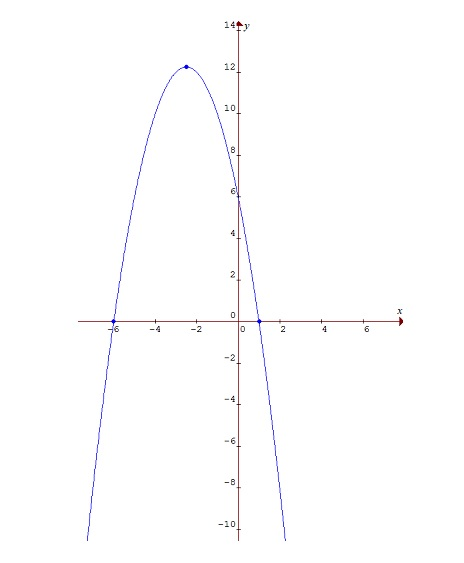
\includegraphics[width=.5\linewidth]{2_elem_rekenvaardigheden_B/inputs/tweedegraadsfuncties3.jpg}
%\caption{Voorbeeld tweedegraadsfuncties: grafische voorstelling}
%\label{fig:tweede:vb} 
%\end{figure}


Tekenverloop:


\begin{tabel}{Voorbeeld tweedegraadsfuncties: tekenverloop}
\begin{tabular}{c||c|c|c|c|c}
	$x$ &  & $-6$ &  & $1$ & \\
	\hline 
	$f(x)$ & $-$ & 0 & $+$ & 0 & $-$\\
\end{tabular}
\label{tab:tweede:vb}	
\end{tabel}

\end{voorbeeld}